\documentclass[convert={density=300,size=1080x800,outext=.png}]{standalone}
\usepackage{xcolor}
\usepackage{graphics, graphicx}
\usepackage{tikz, tkz-graph}
\usepackage{pgf, pgfplots}
\usepackage{graphviz, tkz-berge}
\usepackage{graphics, graphicx}
\usepackage{pstricks, pst-node, pst-tree}

\usetikzlibrary{arrows, petri, topaths}
\usetikzlibrary{shapes}
\usetikzlibrary{arrows.meta}
\usetikzlibrary{positioning,automata}



\begin{document}
		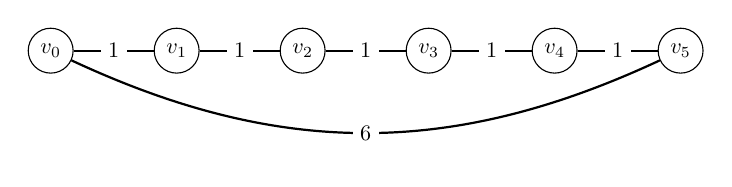
\begin{tikzpicture}[round/.style={circle, draw=black, thin, minimum size=.5mm}, transform shape, scale=0.8]
    \node[round](0) at (0,0){$v_{0}$};
    \node[round](1) at (2,0){$v_{1}$};
    \node[round](2) at (4,0){$v_{2}$};
    \node[round](3) at (6,0){$v_{3}$};
    \node[round](4) at (8,0){$v_{4}$};
    \node[round](5) at (10,0){$v_{5}$};

    \Edge[label=$1$](0)(1)
    \Edge[label=$1$](1)(2)
    \Edge[label=$1$](2)(3)
    \Edge[label=$1$](3)(4)
    \Edge[label=$1$](4)(5)

    \tikzset{EdgeStyle/.style={bend right=25}} %Arestes m�ltiples
    \Edge[label=$6$](0)(5)
    \end{tikzpicture}
\end{document}